\documentclass[a4paper]{article}

\usepackage{template}

\usepackage{pdfpages}

\usepackage[defernumbers=true, datamodel=archiving]{biblatex}
\input{archiving.lbx}

% Be more permissive about line breaks in URLs in the bibliography:
% Credit: https://tex.stackexchange.com/a/134281
\setcounter{biburllcpenalty}{7000}
\setcounter{biburlucpenalty}{8000}

\DeclareBibliographyCategory{formally-peer-reviewed}
\addtocategory{formally-peer-reviewed}{%
  1973-Actors,%
  1984-Linda-and-Friends,%
  emerald:tocs:1988,%
  emerald:tse:1987,%
  emerald:spe:1991,%
  1998-KLAIM,%
  1998-Understanding-code-mobility,%
  2000-QuickCheck,%
  2002-web-based,%
  2004-Context-Awareness-Mobility,%
  2006-Telecoms-QuickCheck,%
  2008-Greening-the-Internet,%
  2009-The-Case-for-VM-Based-Cloudlets,%
  2010-staking-claims,%
  2011-Distributed-Cloud,%
  2011-Validity-and-reliability-in-social-research,%
  2011-Mind-your-language,%
  2012-Fog-Computing-and-Its-Role-in-IoT,%
  2013-mobile-computation-offloading,%
  2013-MCC-A-Survey,%
  2013-Stefik-Siebert-Syntax,%
  2014-A-Survey-of-MCC-Application-Models,%
  2014-Jordan,%
  2015-Borg,%
  2015-Rebooting-MOOC-Research,%
  2016-43-Years-of-Actors,%
  2016-Assessing-the-gold-standard,%
  2016-Fog-Computing-May-Help-to-Save-Energy-in-Cloud-Computing,%
  2016-Programmers-Are-Users-Too,%
  2017-Greening-IoT-with-Fog,%
  2017-Methodological-Irregularities-in-PL-Research,%
  2018-Survey-on-MEC-for-IoT-Realization,%
  2018-Interdisciplinary-PL-Design,%
  2018-MAGA,%
  2018-Understanding-and-misunderstanding-RCTs,%
}

\DeclareBibliographyCategory{phd-theses}
\addtocategory{phd-theses}{%
  2003-PhD-Armstrong,%
  2020-Edge-Computing-for-Extreme-Reliability-and-Scalability,%
  2020-PhD-User-Centerd-Design-of-Principled-PL,%
}

\DeclareBibliographyCategory{books}
\addtocategory{books}{%
  2007-Guide-to-Advanced-Empirical-SE,%
  2008-Seven-Rules-for-Social-Research,%
  2013-HCI-An-Empirical-Research-Perspective,%
  2020-5g-systems-approach,%
}

\DeclareBibliographyCategory{reports}
\addtocategory{reports}{%
  2015-Distributed-Cloud-Dagstuhl,%
  2015-ETSI-MEC-A-key-tech-towards-5G,%
  ericsson-mobrep-2019-wef,%
  2018-Ericsson-TechReview-Distributed-Cloud,%
  2019-ETSI-Developing-Software-for-MEC,%
}

\DeclareBibliographyCategory{media}
\addtocategory{media}{%
  2016-MEC-An-important-ingredient-of-5G-networks,%
  2016-TelecomTV-MEC,%
  2016-Central-office-re-architectured-as-a-data-center,%
  economist2018cars,%
  economist2017drones,%
  economist2017jets,%
  ng2017smartfarming,%
  spiegel2016industrie,%
  spiegel2017industrie,%
}

\addbibresource{references.bib}

\usepackage[numbib]{tocbibind}

\header{%
  course={PhD Project 3rd Semester Status Report},%
  assignment={Mobility-Oriented Programming},%
  subAssignment={A Programming Paradigm for Distributed Mobile Clouds},%
  authors={Oleks Shturmov \texttt{<\href{mailto:oleks@oleks.info}{oleks@oleks.info}>}},%
  affiliation={Department of Informatics\\University of Oslo},%
  shortAffiliation={IFI/UiO},%
  date={December 9, 2020}
}

\newcommand\tm[0]{\textsuperscript{\scriptsize\texttrademark}}
\newcommand\longref[1]{\ref{#1} (page \pageref{#1})}

\usepackage{etoolbox}

\newtheorem{definition}{Definition}

\newtheorem{hypothesis}{Hypothesis}

\newtheorem{conjecture}{Conjecture}

\newtheorem{research-aim}{Research Aim}

\newtheorem{research-objective}{Research Objective}

\newtheorem{scientific-challenge}{Scientific Challenge}

\newtheorem{research-question}{Research Question}

\makeatletter
\renewcommand\tableofcontents{%
    \@starttoc{toc}%
}
\makeatother

\begin{document}

\maketitle

%\input{preface}

\tableofcontents

\pagebreak

\section{Introduction}

\subsection{Project and Scientific Background}

Computing is broadly applicable, in diverse physical environments.

Recent advances in computer architecture, computer networks, and
battery technology, have enabled a proliferation of versatile,
physically mobile, Internet-enabled, computational devices. These
devices collect swathes of data about their surrounding environment,
and increasingly act upon it. Although smartphones are a prime
example, ongoing automation is putting ever more of these devices in
the air\cite{economist2017drones}, on the
roads\cite{economist2018cars}, on factory
floors\cite{spiegel2016industrie, spiegel2017industrie}, in the
fields\cite{ng2017smartfarming}, and into
workshops\cite{economist2017jets}.

Consequently, there are perpetually growing demands for rich digital
services, delivered at low latencies, to devices moving about in
diverse physical environments. These demands have thus far been met by
improving the computational capabilities of the physically mobile
devices, improving (mobile) network performance, and by having elastic
computational resources at centralized server farms (i.e., cloud
computing).

However, it remains prohibitively more expensive to move data over
physical distances, than to perform computation itself. Substantial
gains remain to be leveraged by fundamentally reducing the physical
distances that data must travel. Clearly, many digital services demand
that some data be exchanged over some physical distances.
Never-the-less, a substantial amount of time, wide-area network
traffic, and ultimately, energy, is
wasted\cite{2008-Greening-the-Internet,
2015-Distributed-Cloud-Dagstuhl,
2016-Fog-Computing-May-Help-to-Save-Energy-in-Cloud-Computing,
2017-Greening-IoT-with-Fog}, by concentrating computational resources
at physically centralized locations.

Wide-ranging physical requirements inhibit substantial expansion of
the computational capabilities of the physically mobile devices
themselves --- they must often be small in form factor, light on
weight, and powered by batteries.

% Perhaps a more readily available solution is to provision elastic
% computational resources at more diverse, yet fixed physical locations.
% For instance, our modern digital lifestyle is supported by a large
% number of heterogeneous, networked\footnote{Possibly, but not
% necessarily Internet-enabled.} devices, strategically positioned at
% fixed physical locations. For example, cell-phone towers, telco
% central
% offices\cite{2016-Central-office-re-architectured-as-a-data-center},
% WiFi-hotspots, network switches and routers.  These devices are
% subject to far less stringent physical requirements, having fixed
% power supplies and wired network connections.

% Historically, these devices have used specialized software and
% hardware. However, this approach has proven hard sustain.

% These devices have historically used specialized hardware, and
% software. However, we have grown to realize that this is expensive to
% maintain, especially in the light of dynamic network loads, and that
% there are large business opportunities in 

% this is subject to change with the advent 5G mobile
% networking, and Software-Defined Networking. Increasingly, 

% Possible locations include cell-phone towers, telco central
% offices\cite{2016-Central-office-re-architectured-as-a-data-center},
% factories, office buildings, transport hubs, libraries, retailers,
% restaurants, cafés, bars, etc.

% When a physically mobile device is in need of more computational
% resources, it can refer to some physically closest provider, rather
% than a far-away central server.

A more readily available solution is to provision elastic
computational resources at more diverse physical locations. Elements
of this solution have been considered broadly over the past decade, in
both academia and
industry\cite{2018-Survey-on-MEC-for-IoT-Realization,
2020-Edge-Computing-for-Extreme-Reliability-and-Scalability}. The
approach has bore many names, with subtle variations, including
Cloudlets\cite{2009-The-Case-for-VM-Based-Cloudlets}, Fog
Computing\cite{2012-Fog-Computing-and-Its-Role-in-IoT}, Mobile Cloud
Computing\cite{2013-MCC-A-Survey}, Mobile Edge
Computing\cite{2015-ETSI-MEC-A-key-tech-towards-5G}, and most
recently, Multi-access Edge
Computing\cite{2016-TelecomTV-MEC}\footnote{See also
\url{https://www.etsi.org/technologies/multi-access-edge-computing}.}.
However, the overarching theme has been to deliver on a physically
distributed cloud infrastructure, rather than a centralized
one\cite{2011-Distributed-Cloud, 2015-Distributed-Cloud-Dagstuhl,
2018-Ericsson-TechReview-Distributed-Cloud}, while also supporting the
physical mobility of devices leveraging such
infrastructure\cite{2018-MAGA}:

\begin{definition}[Distributed Mobile Cloud]

\label{def:mobile-cloud}

A distributed mobile cloud infrastructure, is a computational
infrastructure, where elastic computational resources, distributed
over fixed, but diverse physical locations, cater to physically mobile
devices.

\end{definition}

To fully leverage the potential benefits of a distributed mobile
cloud, we must also adapt the way we build applications, to make sure
that they can thrive in this, much more dynamic execution
environment\cite{2014-A-Survey-of-MCC-Application-Models,
2015-Distributed-Cloud-Dagstuhl,
2019-ETSI-Developing-Software-for-MEC}.

A key distinguishing feature is that it is not known at compile-time
where it would be most optimal to place each part of an application.
Optimal placement depends on a multitude of runtime conditions (e.g.,
the current location, and battery charge of mobile devices; various
device and network loads). Furthermore, these conditions change
throughout the lifetime of an application (e.g., mobile devices move),
and it may prove worthwhile to move parts of the application to new
locations, at runtime. This calls for a virtualized address space of
mobile application components, managed in a distributed fashion.

At the same time, component placement cannot be optimal without taking
the needs of the application into account. For instance, to guarantee
a certain level of service, some components must remain co-located, or
maintain some degree of physical proximity, in addition to maintaining
some computational and networking capabilities.  Deriving such
constraints is hard to fathom, without involving the programmers. For
instance, through their use of specialized programming abstractions,
whereby they provide hints and demands to the runtime, as to what
should, or should not move; when, where, and why.

Lastly, applications have something to gain from being aware of their
dynamic operating conditions. For instance, it is common for video
streaming applications to adjust their video quality to the available
network bandwidth. Furtermore, isolating resource-heavy components,
and opportunistically offloading them to other devices, is an active
area of research\cite{2013-mobile-computation-offloading}.

A programming paradigm that collectively addresses the challenges
above, may be referred to as a ``mobility-oriented'' programming
paradigm:

\begin{definition}[Mobility-Oriented Programming]

In a mobility-oriented programming paradigm, an application is
structured in terms of resource-aware, mobile components, subject to
programmer-specified mobility strategies and constraints.

\end{definition} 

The notion of mobility-oriented programming is not
novel\footnote{Although referring to this notion as
``mobility-oriented programming'' is.}. Elements of it have appeared
in the past (e.g., \cite{emerald:tocs:1988},
\cite{1998-Understanding-code-mobility}, \cite{1998-KLAIM},
\cite{2004-Context-Awareness-Mobility}). Previous work has attempted
to propose less verbose and less error-prone primitives for
programming distributed systems in general. However, mobility-oriented
programming has largely remained dormant over the past decade, as we
have witnessed an evolution of needs towards distributed mobile
clouds.

This project rests on a conjecture, that mobility-oriented
programming, adequately construed, can prove to be an \emph{eloquent}
programming paradigm for distributed mobile clouds. This conjecture is
materialized as Hypothesis \ref{hyp:main} on page \pageref{hyp:main}.
First however, a definition of eloquence:

% During that time, we have witnessed two important developments:
% First, there has been an evolution of needs towards distributed
% cloud infrastructures, as outlined above. Second, (centralized)
% cloud computing has matured, and the need to provide elastic
% computational resources, in multi-tenant environments (i.e.,
% centralized server farms), has fueled an evolution of operating
% system-level virtualization, and the emergence of so-called
% ``containers''\cite{2015-Borg}: 

% \begin{definition}[Container]

% \label{def:container}

% A container is a collection of OS-level threads, regarded by the
% operating system as a single logical unit, which may share OS-level
% resources with the rest of the system, or wield over isolated,
% virtualized instances of those resources (e.g., process table, file
% system, network interfaces).

% \end{definition}

% OS-level virtualization can be more light-weight than hardware
% virtualization. For instance, starting a container is a matter of
% spawning a collection of threads, and creating virtualized instances
% of OS-level resources, rather than starting a (virtual) machine, and
% booting an operating system from scratch.

% Perhaps more importantly, containers offer a more fine-grained
% systems structuring primitive, than do virtual machines. Unlike a
% virtual appliance, a container appliance does not need to also house
% an operating system kernel, and otherwise unrelated operating system
% resources (e.g., system files).

% These characteristics have led containers to become not only a
% popular structuring primitive for cloud-based applications, but also
% an important tool in software development. Programmers can use the
% same container appliances in development, testing, and production to
% trivially ensure consistency between these environments; while
% running fundamentally different operating systems in development,
% testing, and production. This eliminates differences in operating
% system, and software configuration as a source of discrepancy
% between these environments.

% Containerized applications communicate across container boundaries
% using interprocess communication. For instance, containers resident
% on the same machine may employ domain sockets, pipes, or message
% queues, while employing standard Internet protocols over network
% sockets for communication across (supposed) machine boundaries.

% The use of interprocess communication, allows for containerized
% applications to be polyglot, where programmers can pick the best
% programming language for each part of their application. However,
% this mode of communication can be highly error-prone, as quite
% often, no static guarantees can be provided across programming
% language boundaries.

% For all their benefits, containers are not well-braced for
% distributed clouds. While it is trivial to transfer a container
% appliance from machine to machine, live container migration remains
% experimental\footnote{See, for example, \url{https://criu.org/}.}.

\begin{definition}[Eloquence]

\label{def:eloquence}

A programming paradigm is considered eloquent for a particular domain,
if we can---with reasonable time and effort---train programmers in
using a programming technology that embodies the paradigm to quickly
deliver, largely error-free, useful, and maintainable applications
within the given domain.

\end{definition}

Of course, what may be considered ``reasonable time and effort'', or
what may be considered a ``quickly delivered'', ``useful'',
``maintainable'', or even ``largely error-free'' application, are
almost purely social questions. It follows, that it is best to apply
methods from social sciences to evaluate eloquence. How does this fit
in the context of a PhD Project in Computer
Science\footnote{Recently, a similarly inclined PhD dissertation was
submitted by Michael J. Coblenz at the Department of Computer Science
at Carnegie Mellon
University\cite{2020-PhD-User-Centerd-Design-of-Principled-PL},
advocating for a user-centered design methodology for principled
programming languages.}?

Firstly, I believe that eloquence should be put on a more rigorous
footing to advance the applicability of programming paradigm research
in practice.  Without evaluations of eloquence, programming paradigms
are rigorously distinguishable only by their conceptual differences,
and how efficient their implementations are. However, those seeking to
reap the benefits of programming paradigm research, typically have a
particular programmer resource at their disposal. It is rudimentary,
to try and make the best use of that resource.

Secondly, I believe that eloquence can be put on a more rigorous
footing, using methods already applied in other fields of Computer
Science. Empirical evaluation, including evaluation of human (e.g.,
user, programmer) factors, is today common-place in the fields of
Human-Computer
Interaction\cite{2013-HCI-An-Empirical-Research-Perspective} and
Software Engineering\cite{2007-Guide-to-Advanced-Empirical-SE}. Less
so in the field of Programming Languages, but this is subject to
ongoing developments\cite{2010-staking-claims,
2016-Programmers-Are-Users-Too,
2017-Methodological-Irregularities-in-PL-Research,
2018-Interdisciplinary-PL-Design}.

Lastly, well-founded evaluation of eloquence cannot proceed without
substantial programming efforts. Today, empirical evaluation is seldom
used to substantiate the design of programming technology. Instead,
designs tend to be driven by disjointly frantic programmer cultures
and market demands. Programming technologies, targeting similar
domains, may well differ in technical maturity, quality of
documentation, available training resources, etc. This makes them
ill-equipped for empirical evaluation, as they initially differ by
many more factors than the factor that we may choose to study.
Controlled experiments cannot be achieved without substantial masking,
re-implementation, and re-writing efforts. This is discussed at depth
in Sections \ref{sec:scientific-challenges} and
\ref{sec:scientific-method}.

\subsection{Main Research Aims and Objectives}

Resting on the above discussion, the main research aim of this project
is to:

\label{research-aim}\newcommand{\researchAim}{\begin{research-aim}
Investigate in-how-far mobility-oriented programming can be an
eloquent programming paradigm for distributed mobile
clouds.\end{research-aim}}\researchAim{}

% To that end, 4 support vectors are considered fundamental to a
% mobility-oriented programming paradigm for distributed clouds:

% \begin{enumerate}[label={(\alph*)}]

% \item \label{aim:location-transparency} That programmers can remain
% oblivious to the exact location of (parts of) data and computation at
% runtime.

% \item \label{aim:resources} That program components can maintain a
% relative capability of retrieving data, and spawning computation at
% runtime.

% \item \label{aim:move} That programmers have the capability to guide
% the runtime on when and where it might be best to move data and
% computation next.

% \item \label{aim:heterogeneity} That data and computation can be
% spread over heterogeneous devices, having different computational
% capabilities.

% \end{enumerate}

% The investigation of the relative benefits of each
% of these forms a separate research objective. 


% To get there, we can employ the following research methodology:
% Begin with an investigation of what makes programming for a
% distributed cloud ineloquent today. Such an investigation is likely
% to result in some informal hypotheses. To make those hypotheses
% concrete, consider a programming technology (or several) that
% explicitly attempts to address those issues, and one (or several)
% that does not. Prove, or disprove, the hypotheses by comparing how
% well programmers fare in solving domain-relevant problems, using the
% respective programming technologies (e.g., in a randomized
% controlled trial).

% In such a methodology, achieving the above aim, is a matter of
% accomplishing the following objectives:

Achieving the above aim is considered to be a manner of accomplishing
the following objectives:

\begin{research-objective}\label{objective:identify}

Identify key elements of eloquence in programming for a distributed
mobile cloud.

\end{research-objective}

% For instance, that programmers can remain oblivious to the exact
% location where a part of their application is executing (i.e.,
% location transparency), or that they can remain aware of the costs
% involved in reaching parts of their application (i.e., resource
% awareness).

Having identified some key elements, we can characterize one, or
several programming technologies that would provide such elements in
practice. Subsequently, objectives
\ref{objective:characterize}--\ref{objective:evaluate} may be
accomplished one, or several times:

\begin{research-objective}[Repeated] \label{objective:characterize}

Characterize a programming technology that
provides the elements of eloquence identified above.

\end{research-objective}

Implementations of the characterized programming technology may exist.
However, they may be outdated, or not suitable for subsequent
eloquence evaluations---they may be tainted by a range of objectives
other than simply addressing the particular element of eloquence in
question.

\begin{research-objective}[Repeated] \label{objective:implement}

Provide an efficient implementation of the programming technology
specified above, amenable to subsequent eloquence evaluation.

\end{research-objective}

While scientific results are achievable through mere characterization
and efficient implementation of novel programming technology alone
(roughly, objectives 2--3), to fully reach the research aim above, we
must finally also:

\begin{research-objective}[Repeated] \label{objective:evaluate}

Evaluate that the programming technology characterized and implemented
above enables programmers to eloquently leverage a distributed mobile
cloud infrastructure.

\end{research-objective}

This last research objective, is expected to result in a considerable
contribution to the research methodology in programming paradigm
research. Never-the-less, to showcase a method for scientific
evaluation of the eloquence of a programming paradigm is not the main
research aim of this project.


\section{Research Questions and Scientific Challenges}

\subsection{Scientific Challenges}

\label{sec:scientific-challenges}

The first obvious challenge is to:

\begin{scientific-challenge} \label{challenge:hypotheses}

Formulate scientifically verifiable hypotheses as to the key elements
of eloquence when programming for distributed mobile clouds.

\end{scientific-challenge}

This is a challenge because distributed mobile cloud computing is in
its infancy. At least, in the sense that there isn't an overabundance
of mature, widely adopted applications, open to scrupulous analyses of
their source code revisions, and bug databases. Furthermore, it is not
straight-forward to interview a representative sample of industry
experts, given the resources available to this project. Of course, we
can leverage the body of hypotheses prevalent in ongoing experimental
work in distributed mobile cloud computing, and distributed computing,
in general. However, since empirical evaluation of eloquence is not
prevalent throughout, these hypotheses may need to be substantially
revised.

\bigskip

Having formulated such hypotheses, we need to evaluate them
scientifically. Since eloquence is a social aspect, it is best to
apply evaluation methods most prevalent in the social sciences. When
applying such methods, it is important to remain vigilant of the many
potential threats to the reliability and validity of their
results\cite{2011-Validity-and-reliability-in-social-research}. The
following discusses some of them.

% \begin{scientific-challenge}

% Devise means to scientifically evaluate the hypotheses relating to the
% eloquence of programming paradigms, while characterising and guarding
% against potential threats to the reliability and validity of such
% evaluations.

% \end{scientific-challenge}

% % There are two main categories of methods in the social
% % sciences---observational and experimental studies.  In observational
% % studies, we observe, but do not alter the population under study. In
% % experimental studies, we administer specific treatments in a
% % controlled fashion, in attempt to measure their effect.
 
Firstly, it is often infeasible to study an entire target population,
including in our case, and so an initial scientific challenge is to:

\begin{scientific-challenge}\label{challenge:representative-sample}

Gather representative samples of the distributed mobile cloud
programmer population, willing to participate in studies.

\end{scientific-challenge}

Furthermore, cultures evolve, populations change, and so social
aspects tend to vary over
time\cite{2008-Seven-Rules-for-Social-Research}. This is true for
programmer culture as well\footnote{For instance, the syntax of
popular languages today differs substantially from the syntax of
popular languages a decade ago.}. Hence, another threat to reliability
and validity stems from working with temporally unstable hypotheses,
or not having a way to test the ``liveness'' of a hypothesis in
different social settings.

\begin{scientific-challenge}\label{challenge:change}

Formulate strategies for verifying that the above hypotheses still
hold in different social settings, and how to spot when they don't.

\end{scientific-challenge}

Another major threat to validity in the social sciences are
confounding factors. This is when factors which we fail to observe, or
control for, happen to be the true cause of particular outcomes.

Perhaps the most prevalent approach to try and mitigate for
confounding factors in the social sciences is to conduct randomized,
controlled trials (RCTs)\cite{2016-Assessing-the-gold-standard,
2018-Understanding-and-misunderstanding-RCTs}. The approach, briefly,
is to randomly split a large population sample, into a control and
treatment group.  Subject to the hypothesis that a particular
treatment has a particular effect on the target population, the
treatment is administered to the treatment group, but not to the
control group. If we subsequently observe the hypothesized effect in
the treatment group, but not in the control group, then this increases
the credibility of the hypothesis.

Randomization however, does not guarantee freedom from confounding
factors---it merely increases the chance of such freedom. Although we
can repeat RCTs, and use larger population samples; it is best to
combine RCTs with other observational studies to ensure
credibility\cite{2018-Understanding-and-misunderstanding-RCTs}. 

Controlled trials, are complicated when dealing with complex
treatments, such as alternative programming paradigms. A programming
paradigm is a mental tool, often greater than the sum of its parts,
used by programmers to conduct creative work. Although randomization
can mitigate for differences in programmer motivation, programmer
efficiency still depends on such ``mundane''\footnote{Often unrelated
to the programming paradigm itself.} things as
syntax\cite{2013-Stefik-Siebert-Syntax}, quality of error
messages\cite{2011-Mind-your-language}, availability of documentation,
and (community) support. It would be ill-advised to directly compare
programming paradigms that differ by such unrelated factors.
Controlling for them, demands that we develop specialized programming
environments for use in our experiments.

\begin{scientific-challenge} \label{challenge:apparatus}

Develop experimental apparatus, in the form of specialized programming
environments, for conducting experiments on human programmers,
including randomized, controlled trials, to evaluate the hypotheses
above.

\end{scientific-challenge}

Use of specialized programming environments, would usually require
additional programmer training, as part of the experiment. Differences
in instruction are another common source of differences in programmer
efficiency. Hence, it is important that the instruction given to the
control group differs from the instruction given to the treatment
group in a controlled way.

\begin{scientific-challenge} \label{challenge:teaching-aids}

Develop teaching aids to ensure consistent programmer training, except
where differences in the training of the treatment and control groups
are demanded by the experiment.

\end{scientific-challenge}

% Observational studies tend to be more prone to such confounding
% factors, since they can only rely on expert knowledge. Experimental
% studies can try to remedy for this by resorting to
% \emph{randomized}, controlled trials (RCTs). For instance, where the
% population sample is randomly split into a treatment and a control
% group, with only the former being administered a treatment. By
% assigning individuals to these groups at random, we increase our
% chances to not fall prey to some confounding factors which we failed
% to control for.

% After an initial success in medicine, randomized, controlled trials
% (RCTs) seem to be well on their way to becoming a ``gold
% standard''\cite{2016-Assessing-the-gold-standard} in the social
% sciences as well\cite{2018-Understanding-and-misunderstanding-RCTs}.

% Overall, this project involves both exploratory research, and
% confirmatory research. Such a distinction can be drawn between
% Research Objective 1 and Research Objectives 2--4.

% The trouble with doing exploratory research in matters pertaining to
% social aspects (e.g., eloquence), is how to study a sufficiently
% representative sample of the target population. Distributed mobile
% cloud computing is in its infancy.Whatever
% distributed mobile cloud applications there are, are themselves
% experimental.

% Distributed mobile cloud applications are in their infancy.

% Neither is it straight-forward to interview a
% representative sample of industry experts, given the resources
% available to this project.

% To identify eloquent programming techniques for distributed
% mobile clouds in a scientific manner, we must adopt an exploratory
% research methodology:

% Having formulated such hypotheses, we can evaluate their validity
% through empirical evaluation with human programmers.

% Having formulated such hypotheses, we need to evaluate their
% validity empirically. For instance, using of \emph{rapid
% prototyping}, \emph{A/B-testing}, and \emph{discount usability
% evaluation}\cite{2016-Programmers-Are-Users-Too}, and
% \emph{randomized controlled trials}. Each such empirical evaluation
% would involve roughly the following steps:

% \begin{enumerate}

% \item Draw a sample of the distributed mobile cloud programmer population.

% \item Divide the population randomly into equally-sized groups.

% \item Hand each group, each their own variant of otherwise the same
% programming technology, the variants varying only in the elements
% under test.

% \item Pose equivalent programming problems, which might elucidate the
% eloquence/ineloquence of the various variants.

% \item Compare the eloquence with which the groups solve the given
% problems.

% \end{enumerate}

% Taking this approach means that we cannot immediately use existing
% programming technology that supposedly provides an element of
% eloquence, and compare it with technology that supposedly does not.
% Existing programming technologies may vary in many more factors, than
% the way in which that they address a particular element of eloquence.
% They may vary in popularity, maturity, availability and quality of
% documentation, training material, etc. We must control for all these
% factors to arrive at some scientifically valid distinctions.

% The obvious way to do so is to re-implement, and mask existing
% programming technology, to provide new documentation, new training
% material.


\subsection{Research Questions}

% In a distributed mobile cloud, both data and computation are mobile.

% Without loss of generality, we can refer to the lumps of data and
% computation thus moving about as ``objects'':

% \begin{definition}[Object]

% An object is a conglomeration of data and computation; a unit of
% mobility in a distributed mobile cloud.

% \end{definition}

% These objects move about among a collection of ``hosts''.

% \begin{definition}[Host]

% A host is a network-addressable (virtual) machine capable of serving
% as the location of an object in a distributed mobile cloud. An object
% is ``located'' at a given host in the sense that its data is stored
% at, and computation is effectuated on that machine.

% \end{definition}

% When an object is in transit from host to host, no computation can
% take place.

% \begin{definition}[Distributed Mobile Cloud (cont.)]

% A distributed mobile cloud consists of a number of hosts, where some
% of them may be physically mobile. The set of available hosts is not
% fixed, new hosts may appear, existing hosts may disappear, and hosts
% may temporarily become unavailable.

% \end{definition}

% Although the scientific challenges above focus heavily on the last
% research objective above (number \ref{objective:evaluate}), the main
% research questions of this project span all of the research
% objectives.

Extrapolating from the background studies conducted in this project so
far, the subject work of this project rests on the following
hypothesis:

\begin{hypothesis}

\label{hyp:main}

The following characteristics are elementary to eloquent distributed
mobile cloud programming:

\begin{description}

\item[Location Transparency] --- programmers can remain oblivious to
the exact location of (parts of) data and computation at runtime.

\item[Resourcefulness] --- program components can maintain some
relative capability of retrieving data, and performing computation at
runtime.

\item[Context-Awareness] --- program components can act aware of their
current execution environment, and react to changes to it.

\item[Coordinated Mobility] --- programmers can guide the runtime on
when and where it might be best to move data and computation next.

\item[Heterogeneity] --- data and computation can be spread over
heterogeneous devices, having different computational capabilities and
software.

\end{description}

\end{hypothesis}

To address elements of this hypothesis in a scientific manner, the
following research questions address them more concretely.

\bigskip

Many contemporary distributed programming systems draw an explicit
distinction between local and remote procedure calls. Some however,
make no such syntactic distinction (e.g.,
Emerald\cite{emerald:tocs:1988, emerald:tse:1987, emerald:spe:1991},
Erlang\cite{2003-PhD-Armstrong}), and refer to this characteristic as
``location transparency''. The eloquence of the presence/absence of
location transparency has not been backed by scientific evidence.

It would seem however, that the most eloquent approach is somewhere
in-between: We would like to remain oblivious to the exact location of
objects, in the face of mobility. However, we also need to keep a tab
on how these objects move about, so that some physical proximity is
maintained among them.

\begin{research-question}[Location Transparency and Coordinated Mobility]

How does the presence/absence of location transparency influence the
eloquence of a programming technology for a distributed mobile cloud?
If there are drawbacks to location transparency, could some
coordinated mobility primitives help alleviate them?

\end{research-question}

The set of resources available to any given object in a distributed
mobile cloud is dynamic. It cannot be determined at compile-time, and
may change throughout the lifetime of an object. Never-the-less, to
guarantee a certain level of service, individual objects need a
certain set of resources to operate.

The needed set of resources can be characterized by the programmer
(e.g., through their use of specialized programming abstractions). If
the runtime cannot, or can no longer deliver the necessary resources
at a given location, it might be worthwhile to move the object
elsewhere.
 
\begin{research-question}[Resourcefulness, Context-Awareness, and
Coordinated Mobility]

What are some eloquent means for programmers to characterize the
resources necessary for the proper functioning of an object in a
distributed mobile cloud?  Subsequently, how can programmers
eloquently specify what should happen when those resources cannot, or
can no longer be delivered at the current object location?

\end{research-question}

The devices providing the computational infrastructure in a
distributed mobile cloud are highly heterogeneous. They involve
machines in large, and small data centers, nearby commodity servers,
physically mobile devices, elements of the mobile network
infrastructure (e.g., base stations, central
offices\cite{2016-Central-office-re-architectured-as-a-data-center,
2020-5g-systems-approach}), among others.  These devices differ in
both their hardware resources, and their software stacks. Supporting
object mobility in such a diverse computational infrastructure is
challenging in its own right.

Furthermore, programmers often would like to use the best tool for
each part of their job. In particular, a modern digital service is
often built from components written in a myriad of different
programming languages. It would be feeble to attempt to deliver a
single programming language for programming distributed mobile cloud
applications, in general.  Instead, a language that otherwise
addresses the characteristics outlined above, should come with good
language interoperability options. Allowing programmers to employ
existing components, written in other languages, and to write new
components in languages most suitable for those components.

\begin{research-question}[Heterogeneity]

How can we eloquently support the execution of heterogeneous software
across a network of heterogeneous devices, as we see in a distributed
mobile cloud?

\end{research-question}

% The aforementioned literature will often go on to suggest the design
% and implementation of a novel programming paradigm, in attempt to
% address the supposed sources of ineloquence. The suggested programming
% paradigm may or may not be picked up by the general public, and may or
% may not reach a certain level of maturity.

% Existing programming paradigms that may address the same source of
% ineloquence. However, they are also likely to vary by many more
% factors than the source of ineloquence itself. Hence, we cannot
% trivially compare them, in terms of how well they fare in addressing
% the source of ineloquence.

% Instead, we need to employ rapid prototyping, re-design and
% re-implement these paradigms, such that only a controlled number of
% factors vary.

% \begin{scientific-challenge}[Design]

% Design programming paradigms in attempt to address the sources of ineloquence 

% This is related to Research Objective \ref{objective:characterize}.

% \end{scientific-challenge}

% \begin{scientific-challenge}[Implementation]

% This is related to Research Objective \ref{objective:implement}.

% \end{scientific-challenge}

% \begin{scientific-challenge}[Evaluation]

% This is related to Research Objective \ref{objective:evaluate}.

% \end{scientific-challenge}


% A substantial scientific challenge stems from the desire to evaluate
% the eloquence of programming technologies. As defined on page
% \pageref{def:eloquence}, eloquence is a social aspect. As such, it is
% perhaps best evaluated using methods from the Social Sciences, where
% we construct falsifiable hypotheses, about how certain societies
% behave, and subject these hypotheses to empirical evaluation.

% \begin{scientific-challenge}
% 
% Representative sample
% 
% \end{scientific-challenge}
% 
% The fundamental, operating hypothesis of this projects is that:
% 
% \begin{hypothesis}
% 
% \label{hyp:main}
% 
% Programmers need substantial support from the underlying programming
% environment to eloquently leverage the potential benefits of a
% distributed cloud infrastructure. In particular, the required support
% vectors are:
% 
% \begin{enumerate}[label={(\alph*)}]
% 
% \item \label{hyp:location-transparency} That programmers can remain
% oblivious to the exact location of (parts of) data and computation at
% runtime.
% 
% \item \label{hyp:resources} That program components can maintain a
% relative capability of retrieving data, and spawning computation at
% runtime.
% 
% \item \label{hyp:move} That programmers have the capability to guide
% the runtime on when and where it might be best to move data and
% computation next.
% 
% \item \label{hyp:heterogeneity} That data and computation can be
% spread over heterogeneous devices, having different computational
% capabilities, powered by heterogeneous software.
% 
% \end{enumerate}
% 
% \end{hypothesis}
% 
% This hypothesis will be subject to evaluation, and perhaps, evolution,
% throughout the project.
% 
% \subsection{Research Questions}
% 
% The research questions are organized such that they successively
% address the elements of Hypothesis \ref{hyp:main} above.
% 
% Sub-hypothesis \ref{hyp:location-transparency} refers to a design
% principle that has been widely employed in programming technologies
% for distributed systems before: \emph{location transparency}[?].
% Unfortunately, related scientific literature has, at best, presented
% anecdotal evidence in favor of it, and it has also been anecdotally
% criticised[?].
% 
% \begin{research-question}[Location Transparency]
% 
% How does location transparency contribute to the eloquence of a
% programming technology for a distributed cloud?
% 
% \end{research-question}
% 
% Sub-hypothesis \ref{hyp:resources} refers to the ability of
% programmers to remain aware of the resources available to them. Either
% local resources, or resources available over the network. This too
% refers to a design principle that has been widely prevalent in
% academic literature: \emph{resource-aware programming}[?]. As with
% location transparency, the evidence of the relative merits of
% resource-aware programming, remains anecdotal.
% 
% \begin{research-question}[Resource-Aware Programming]
% 
% How does resource awareness contribute to the eloquence of a
% programming technology for a distributed cloud?
% 
% \end{research-question}
% 
% Although resource-aware programming is an active area of research, it
% tends to focus on enabling programmers to write application components
% that do not exceed certain resource limits. Another approach is to let
% programmers roam free, but constrain their components, and provide
% handlers for when they fail to meet those constraints. Hence, the
% runtime would forcefully suspend the offending components, and refer
% to the handlers until further notice.
% 
% I conjecture that this sort of ``resource-constrained programming''
% could fit naturally in a programming technology for distributed
% systems. Here, it is already natural to program with timeouts, to
% address the unreliable nature of networks of computers.  We could
% treat a component that exceeds the resources available to it, as a
% component that has ``unexpectedly'' become unavailable.
% 
% \begin{research-question}[Resource-Constrained Programming]
% 
% How does resource-constrained programming contribute to the eloquence
% of a programming technology for a distributed cloud?
% 
% \end{research-question}
% 
% Sub-hypothesis \ref{hyp:move} also refers to an ability that we have
% seen in programming languages for distributed systems before[?]. Here,
% programmers are given primitives that allow them to guide the runtime
% on when and where to move data and computation.
% 
% \begin{research-question}[Directed Mobility]
% 
% How does having the ability to direct the mobility of data and
% computation contribute to the eloquence of a programming technology
% for a distributed cloud?
% 
% \end{research-question}
% 
% Overall, resource-aware and resource-constrained programming, and
% directed mobility, adequately combined, can also address
% sub-hypothesis \ref{hyp:heterogeneity}. Truly eloquent programming for
% a distributed cloud however, may require a non-trivial combination of
% the above design principles. The above research questions separate
% them out however, to highlight the importance of investigating the
% relative merits of each one individually.
% 
% \subsection{Scientific Challenges}
% 
% \label{sec:scientific-challenges}
% 
% \begin{scientific-challenge}
% 
% Evaluate the eloquence of a programming technology.
% 
% \end{scientific-challenge}
% 
% % \begin{enumerate}
% 
% % \item Programming technology tends to mature without a scientific
% % regard for human factors. As we begin to question this, we are faced
% % with the fact that mature programming technology can be easier to
% % learn and employ due to an overabundance of readily available training
% % material.
% 
% % This however, does not mean that programmers trained in this
% % technology will quickly deliver useful, maintainable, or largely
% % error-free applications in any particular domain.
% 
% % \item Programming technology tends to evolve in a particular social
% % context. While it may grow to become eloquent in that context,
% % it may not appear so in a different one. That appearance might, or
% % might not be justified.
% 
% % For instance, a programming technology might have gone out of favor,
% % but if endowed with another name, more timely syntax, and training
% % material, it might prove eloquent in a more contemporary social
% % context.
% 
% % \item Replication
% 
% % \end{enumerate}
% 
% 
% 
% \subsection{Status Regarding Reaching Beyond State-of-the-Art}
% 
% \begin{itemize}
% 
% \item Identified mobility-oriented programming as a programming
% paradigm.
% 
% \item Re-implemented Emerald to have:
% 
% \begin{itemize}
% 
% \item Flexible compiler architecture, to make it straight-forward to
% experiment with novel and alternative syntax and semantics.
% 
% \item BEAM as a back-end.
% 
% \end{itemize}
% 
% \end{itemize}


\subsection{Status regarding reaching beyond the state of the art}

The onset for this project was to explore what the ideas inherent in
the Emerald programming language\cite{emerald:tocs:1988,
emerald:tse:1987, emerald:spe:1991} might be good for today, and
looking into the future. Emerald is a general purpose programming
language, devised in the early 1980s in an academic attempt to address
the challenges inherent in programming distributed systems, as they
were projected to be at the time. Emerald has since gained little
adoption, beyond small academic circles.

I have identified ``mobility-oriented programming'' as the general
programming paradigm first embodied by the Emerald programming
language. This paradigm contrasts itself with what might be called
``message-oriented programming'', such as embodied by the actor
model\cite{1973-Actors, 2016-43-Years-of-Actors}, and the Erlang
programming language\cite{2003-PhD-Armstrong}, and ``tuple-space
programming'', such as embodied by the Linda programming
language\cite{1984-Linda-and-Friends}: In mobility-oriented
programming, programmers are more concerned with the mobility of
system objects, and less, or equally, concerned about the
communication among those objects.

Mobility-oriented programming is suitable in a domain where system
objects will naturally move about, and it is important to control
their mobility to ensure some intended functioning of the application.
I have identified distributed mobile clouds as one suitable domain
of applications for such a programming paradigm. See the introduction
for a discussion of this domain.

To scientifically evaluate in-how-far such a programming paradigm is
suitable for this domain, I have formalised\footnote{In the social,
rather than mathematical sense of this word.} the notion of
programming paradigm eloquence, and designed a methodology for
evaluating it (see also Section \ref{sec:scientific-method}).

To technically enable such evaluations, I have begun work to
implement:

\begin{enumerate}

\item A modern Emerald compiler, affording experimentation with more
modern syntax for Emerald, and better error messages.

\item A modern Emerald runtime on top of BEAM, a popular Erlang
Runtime System implementation. This would allow us to run Emerald code
on-par with Erlang code.

\end{enumerate}

\subsubsection{Publications (and lack thereof)}

In order to canvas cutting edge approaches to connecting heterogeneous
components (Research Question 3), I have devised a novel
``Interconnecting Code Workshop'' at the <Programming>
conference\footnote{\url{https://programming-conference.org/}}. I have
organized two iterations of the workshop in
2019\footnote{\url{https://2019.programming-conference.org/track/icw-2019-papers}}
and
2020\footnote{\url{https://2020.programming-conference.org/home/icw-2020}},
together with my main advisor, Eric Jul. This serves as proof of the
scientific relevance of Research Question 3.

I have also had a talk approved at another workshop at the
<Programming> 2020 conference, namely MoreVMs'20 --- Workshop on
Modern Language Runtimes, Ecosystems, and VMs. The talk was entitled
``Towards Modern Runtime Support for an Object-Based Distributed
Programming Language'' and I submitted an
abstract\footnote{\url{https://2020.programming-conference.org/details/MoreVMs-2020-papers/9/Towards-Modern-Runtime-Support-for-an-Object-Based-Distributed-Programming-Language-}}.
However, I did not give the talk due to circumstances related to
COVID-19. 


\section{Scientific Method}
\label{sec:scientific-method}

The general approach is iterated experimental analysis, engineering,
and evaluation of tools for programming modern distributed
applications.  The following subsections, cover the steps involved in
every such iteration in more detail.

\subsection{Analysis}

The objective of this project is to reduce the engineering effort
required to build modern, heterogeneous distributed systems. This
requires a systematic analysis of how such systems are built today,
and to identify key hurdles in this present-day engineering practice.

Luckily, modern distributed systems software is often open source,
subject to reversion control, and open bug-tracking. This means that
both various versions of an application, its past and present hurdles,
its technical documentation, and an account of its (ongoing)
development, are often directly available for systematic study. The
quantity and quality of these resources may vary considerably across
applications, but far more data is readily available for open-source,
rather than closed-source applications.

Reviewing source code alone does not always give sufficient insight
into real-world system diversity, and runtime behaviour --- monitoring
real-world applications, is an important alleyway for field-work.
However, this can prove challenging as many such systems are
commercial in nature, and data about their runtime behaviour may carry
business value.

Sometimes, real-world workloads can be reliably simulated, based on
public data about system diversity in real-world applications. For
instance, the diversity of handheld devices, and associated operating
systems, that ambitious handheld applications should target, is often
a public statistic.

\subsection{Engineering}

Based on observations of the hurdles of real-world distributed systems
programming, I intend to design and implement programming environments
to try and alleviate some of these. This is a largely creative
process, requiring a considerable engineering effort in its own right.
It involves analysing, using, and composing existing programming
languages, runtime systems, libraries, and frameworks, to form new
ones.

\subsection{Evaluation}

To verify that the programming environments thus engineered tackle
some of the above problems, it is imperative to try and re-implement
the systems studied previously, with the explicit intent to compare
the implementations, subject to real-world workloads.

One way to do this in the context of a existing application, is by
setting up a proxy in front of the original service, such that
requests are funneled to both the original implementation, and the
experimental one. The response from the experimental implementation is
logged for analysis, while the user receives the response from the
original implementation, as before. This is one way to test that an
experimental implementation meets certain requirements under a
real-world workload.

However, since the scientific result in question also has to do with
the necessary engineering effort, there are some human factors that
have to be taken into account during an evaluation:

\begin{enumerate}

\item A person that has seen, or worked on the original
implementation, might forego some of the engineering effort during a
re-implementation in another programming environment, already knowing
how to meet certain requirements in the original programming
environment.

\item A person that has not seen any implementation, asked to make
both, might be affected either way by first using one, or the other
programming environment.

\item A person that knows the original programming environment, might
be hindered in quickly understanding the new programming environment,
or conversely, be better equipped to understand the new programming
environment, than a person that is familiar with neither.

\end{enumerate}

One way to tackle all of these challenges at once would be to:

\begin{enumerate}

\item Attract a representative number of programmers that do not have
familiarity with engineering the original application, and are
familiar with neither programming environment (e.g., university
students).

\item Split them up into two representative groups, and train each in
a different programming environment.

\item Present them with the requirements of the original application,
and ask to implement the original application in the taught
environment.

\item Finally, train them in the other programming environment, and
ask them to reimplement the application in the other environment.

\end{enumerate}

This is quite an elaborate level of rigour. A level of rigour seldom
seen in programming language design, as evidenced by the only recent
discovery of Evidence-Based Programming-Language Design
\cite{dagstuhl18061}. However, it does seem to universally address the
human factors above, and would also provide empirical data on
in-how-far the programming environments are easy to teach, easy to
learn, and how error-prone they are for newcomers.


\section{Ethics}

This project advocates for the use of empirical evaluation involving
humans. In accordance with University of Oslo
recommendations\footnote{\url{https://www.uio.no/english/for-employees/support/research/research-data-management/data-management-plan/index.html}},
a Data Management Plan will be submitted to the Norwegian Centre for
Research Data (NSD). A draft of the Data Management Plan is attached
as Appendix \ref{app:nsd}. However, this form alone would not cover
all the necessary ethical considerations. The following covers what
remains.

Participants will engage in specially crafted programming courses,
subject to the promise that this will improve their knowledge, skills,
and competences in a particular domain. It is imperative that this
promise is delivered upon.

Furthermore, to evaluate the eloquence of a programming paradigm, we
must experiment with what turn out to be ineloquent techniques. What
is eloquent and what is not, only becomes apparent at the end of the
experiment. The solution to this problem is to have all participants
learn all the paradigms being experimented with, before the end of the
experiment, and to inform them of the results of the experiment.

For instance, if we are comparing two paradigms, A and B, and
conducting an RCT, with two groups, X and Y; we can proceed as
follows:

\begin{enumerate}

\item Let group X learn paradigm A, while group Y learns paradigm B.

\item Ask both groups to do the same task using each their paradigm.

\item Let group X now learn paradigm B, while group Y learns paradigm A.

\item Ask both groups to do the same task using each their paradigm.

\item Inform groups X and Y of the results of the experiment, so that
they know which paradigm turned out to be the most eloquent.

\end{enumerate}

This way, by the end of the experiment, no group is left unfairly
trained in what turns out to be an ineloquent programming paradigm.


\section{Changes in the Project}

Compared to the original project
description\footnote{\url{https://github.com/oleks/phd/releases/download/pre-signed-project-description/oleks-phd-project-description.pdf}},
there is now less focus on re-implementing or maturing Emerald, and
more on evaluating the programming paradigm originally afforded by it,
in general. Distributed Mobile Clouds are identified as the particular
contemporary domain of applications where Emerald, or variants of it,
may prove their worth.


\section{Project Plan}

\begin{enumerate}

\item Design and implement a programming language workbench for
experimenting with mobility-oriented programming contrasted with other
programming paradigms for distributed mobile cloud applications.

This is expected to result in scientific contributions in the field of
programming language design and implementation. Possible venues for
publication include <Programming>, ECOOP, POPL, PLDI, and ETAPS conferences.

This is in progress.

\item Design and implement a course on ``Programming Paradigms for
Distributed Mobile Cloud Programming''.

Focus on online content delivery and automated grading (i.e., build a
MOOC). This enables large samples of the target population to
participate, and complete the course. It also enables controlled
variability in what is taught to selected groups in the experiment.

This is expected to result in scientific contributions in terms of how
distributed programming exercises can be reliably graded
automatically. To this end, I plan to employ property-based
testing\cite{2000-QuickCheck, 2006-Telecoms-QuickCheck}, with adequate
extensions for stating properties about distributed (mobile cloud)
systems. Possible venues for publication include ACM Learning at
Scale, PLATEU.

This is in progress.

\item Run multiple iterations of the MOOC, report on the results, and
experiences with the research methodology. This too is expected to
result in scientific contributions. Possible venues for publication
include <Programming>, PLATEU, ECOOP, POPL, PLDI, and ETAPS
conferences.

\end{enumerate}

The current formal trajectory is to finish by November 30, 2021. If
the above work is completed by that time, most of the above may well
be complete, but will probably not yet be published. I have begun
investigating possibilities for formal extensions of this deadline.

% \begin{description}
% 
% \item[September 2020 -- November 2020]\hfill
% 
% \begin{itemize}
% 
% \item Seek feedback on the design of experiments for the evaluation of
% eloquence of programming models
% 
% \end{itemize}
% 
% Potential venues for paper submission:
% 
% \begin{itemize}
% 
% \footnotesize
% 
% \item PLATEAU 2021
% 
% \item European Joint Conferences on Theory \& Practice of Software
% (ETAPS) 2021
% 
% \item The Art, Science, and Engineering of Programming (<Programming>)
% 2021
 
% \item Programming Languages Design and Implementation (PLDI) 2021
% 
% \item International Conf. on Ambient Systems, Networks and
% Technologies (ANT) 2021
% 
% \item International Conf. on Emerging Data and Industry 4.0 (EDI40)
% 2021
% 
% \end{itemize}
% 
% \item[December 2020 -- February 2021]\hfill
% 
% Potential venues for paper submission:
% 
% \begin{itemize}
% 
% \footnotesize
% 
% \item European Conference on Object-Oriented Programming (ECOOP) 2021
% 
% \item USENIX Annual Technical Conference (USENIX ATC) 2021
% 
% \item Workshop on Modern Language Runtimes, Ecosystems, and VMs
% (MoreVMs) 2021
% 
% \item International Conference on Languages Compilers, Tools and
% Theory of Embedded Systems (LCTES) 2021
% 
% \end{itemize}
% 
% \item[March 2021 -- May 2021]\hfill
% 
% Potential venues for paper submission:
% 
% \begin{itemize}
% 
% \footnotesize
% 
% \item International Conference on Functional Programming (ICFP) 2021
% 
% \item International Conference on Types for Proofs and Programs
% (TYPES) 2021
% 
% \item International Conf. on Mobile Systems and Pervasive Computing
% (MobiSPC) 2020
% 
% \item Onward! 2021
% 
% \item CurryOn 2021
% 
% \item OOPSLA 2021
% 
% \item ICOOOLPS 2021
% 
% \item Erlang 2021
% 
% \item International Workshop on Context-Oriented Programming (COP)
% 2021
% 
% \end{itemize}
% 
% \item[June 2021 -- August 2021]\hfill
% 
% Potential venues for paper submission:
% 
% \begin{itemize}
% 
% \footnotesize
% 
% \item The Art, Science, and Engineering of Programming (<Programming>)
% 2022
% 
% \item International Conference on Software Language Engineering (SLE)
% 2021
% 
% \item PLATEAU 2022
% 
% \end{itemize}
% 
% \item[September 2021 -- November 2021]\hfill
% 
% \begin{itemize}
% 
% \item Write dissertation
% 
% \end{itemize}
% 
% \end{description}


\section*{References}

\nocite{*}

\printbibliography[%
  title={Formally Peer-Reviewed},%
  category=formally-peer-reviewed,%
  heading=subbibliography%
]

\printbibliography[%
  title={PhD Theses},%
  category=phd-theses,%
  heading=subbibliography%
]

\printbibliography[%
  title={Books},%
  category=books,%
  heading=subbibliography%
]

\printbibliography[%
  title={Reports},%
  category=reports,%
  heading=subbibliography%
]

\printbibliography[%
  title={Media},%
  category=media,%
  heading=subbibliography%
]

\pagebreak

\appendix

\section{Terminology}\label{app:terminology}

This document is written in accordance with the ``Guidelines for third
semester evaluation of Ph.D.-candidates at the Department of
Informatics
(IFI)''\footnote{\url{https://www.mn.uio.no/ifi/english/about/organisation/phd-committee/for-phd-candidates/3rd-semester-reporting-ifi-19.03.2018.pdf}.}.

Among other things, the guidelines ask the Ph.D.-candidate to list:

\begin{itemize}

\item Main research aims and objectives

\item Scientific challenges

\item Research questions

\end{itemize}

To state these as clearly and unambiguously as possible, this document
uses a writing style reminiscent of Mathematics and Theoretical
Computer Science---it uses typographically distinct, enumerated,
categorised blocks.

For instance, on page \pageref{research-aim}, we have:

\setcounter{research-aim}{0}

\researchAim{}

Throughout the document there are blocks like ``Research Aim 1'',
``Research Objective 2'', ``Scientific Challenge 3'', and ``Research
Question 4''. These are reminiscent of what the guidelines ask for.
However, there are also blocks that underpin them (e.g., ``Definition
1''). The purpose of this appendix is to define the blocks employed
throughout this document. In-so-doing, I also hope to clarify my
reading of the guidelines.

\bigskip

The purpose of a block is to state something as clearly, and
unambiguously as possible. It is common therefore, to have a
progression of blocks, building conceptually on one another, starting
with blocks stated in terms which can be assumed as clear and
unambiguous to the target audience. The progression employed in this
document is as follows:

\begin{description}

\item[Definition] \hfill

An explanation and demarcation of a key term to be employed in latter
text and blocks.

\item[Research Aim] \hfill

A broad statement about a desired outcome of the research project.

There may be multiple aims to a research project.

\item[Research Objective] \hfill

A broad statement about a step which, if taken, would bring us closer
to achieving a desired outcome.

We may need to accomplish multiple research objectives, to achieve a
particular desired outcome.

\item[Scientific Challenge] \hfill

An aspect of a research objective, which is important to consider in
order to achieve the objective in a scientific manner.

Scientific challenges motivate the formulation of the research
questions, and the subsequent research methodology and research
methods.

\item[Research Question] \hfill

A specific question which, if answered in a scientific manner, would
bring us closer to accomplishing a research objective.

We may need to answer multiple research questions, to accomplish a
particular research objective.

\end{description}


\section{Data Management Plan Draft}

\label{app:nsd}

The draft that you see on the following pages is to be submitted to
the Norwegian Centre for Research Data (NSD).

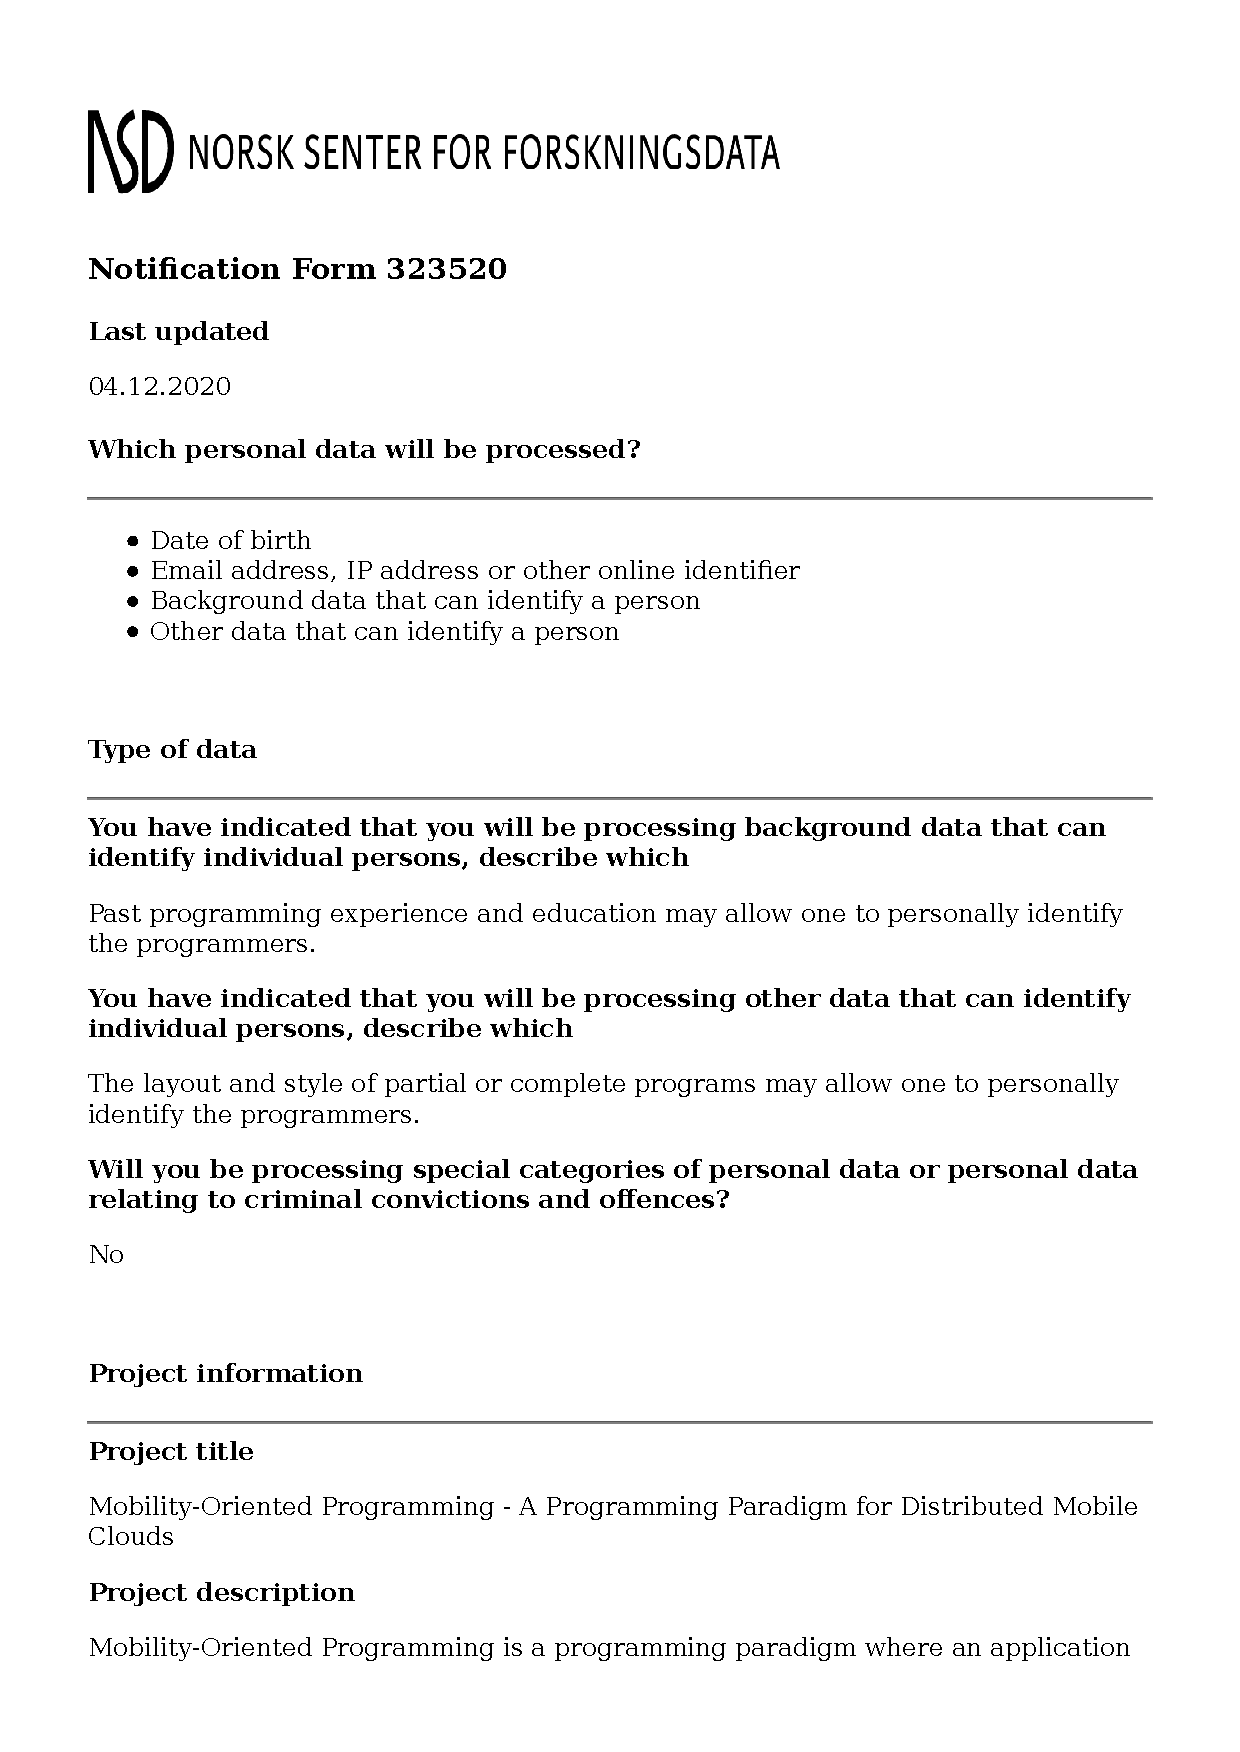
\includepdf[%
  pages=-,%
  width=1.2\textwidth,%
  pagecommand=\thispagestyle{fancy}%
]{2020-12-04-NSD-draft.pdf}


\end{document}
